\section{从 RoPE 相位到答案失效}
\label{sec:mechanism}

\subsection{第一层：固定内容与距离依赖分数}

RoPE 将每个注意力头的维度划分为 $d/2$ 个二维对。对于第 $i$ 个二维对，令
\begin{equation}
  \omega_i=\theta^{-2i/d},\qquad
  \preq_i=\begin{bmatrix}q_{i,x}\\q_{i,y}\end{bmatrix},\qquad
  \prek_i=\begin{bmatrix}k_{i,x}\\k_{i,y}\end{bmatrix}.
\end{equation}
由于旋转构成一个群，
\begin{equation}
  (\Rope_t\preq)^{\top}(\Rope_j\prek)
  =\preq^{\top}\Rope_{j-t}\prek
  =\preq^{\top}\Rope_{-\Delta}\prek.
  \label{eq:relative-rope}
\end{equation}
展开其中一个二维对，可得
\begin{align}
  s_i(\Delta)
  &=A_i\cos(\Delta\omega_i)+B_i\sin(\Delta\omega_i),
  \label{eq:pair-score}\\
  A_i&=q_{i,x}k_{i,x}+q_{i,y}k_{i,y},\qquad
  B_i=q_{i,x}k_{i,y}-q_{i,y}k_{i,x}.
\end{align}
等价地，令 $\rho_i=\sqrt{A_i^2+B_i^2}$ 且 $\psi_i=\operatorname{atan2}(B_i,A_i)$，则
\begin{equation}
  s_i(\Delta)=\rho_i\cos(\Delta\omega_i-\psi_i).
  \label{eq:amplitude-phase}
\end{equation}
内容向量决定振幅与偏好相位，而位置提供相位偏移。因此，一个对语义有用的二维对可能在某一距离上作出正贡献，却在另一距离上作出负贡献。完整注意力头的 logit 为 $s^R(\Delta)=d^{-1/2}\sum_i s_i(\Delta)$；它是有限个振荡项的混合，而非单调的距离惩罚。

若插入 $m$ 个 filler token，使查询后移而键保持不变，则第 $i$ 个二维对的精确变化为
\begin{align}
  \delta s_i
  &=2\sin\!\left(\frac{m\omega_i}{2}\right)
  \left[
  -A_i\sin\!\left(\frac{(2\Delta+m)\omega_i}{2}\right)
  +B_i\cos\!\left(\frac{(2\Delta+m)\omega_i}{2}\right)
  \right],
  \label{eq:pair-delta}\\
  |\delta s_i|
  &\le 2\rho_i\left|\sin\!\left(\frac{m\omega_i}{2}\right)\right|.
  \label{eq:pair-bound}
\end{align}
高频会提高局部敏感度，但只有内容振幅 $\rho_i$ 较大的频率对才具有重要影响。因此，仅由 RoPE 本身既不能推出“高频意味着局部注意力头”，也不能推出“越长必然越差”。

\begin{figure}[t]
  \centering
  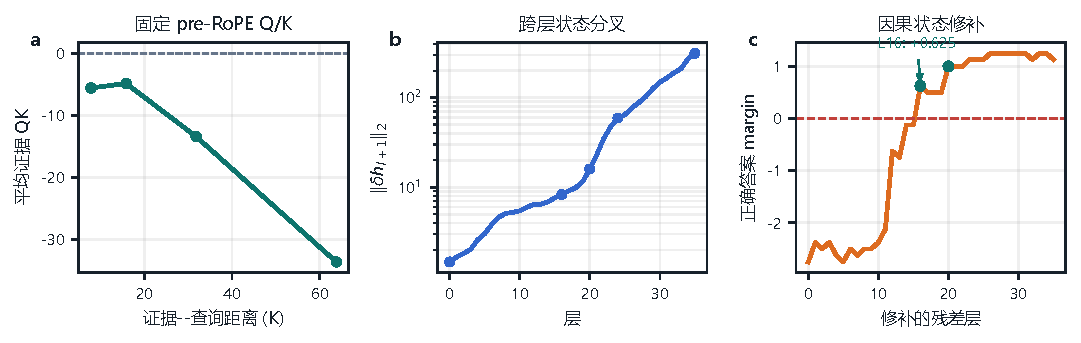
\includegraphics[width=\linewidth]{figures/mechanism_evidence_zh.pdf}
  \caption{Qwen3-8B 上的机制证据。\textbf{左：}在 pre-RoPE Q/K 完全相同的条件下，实测第一层金标准 QK 随距离改变；由 64 个二维对组成的解析和以 $1.98\times10^{-3}$ 以内的误差将其重构。\textbf{中：}一个包含 64 个 token 的诊断扰动在第 0 层产生非零残差差异，且该差异随深度增长。\textbf{右：}在中间层用成功状态替换失败运行的残差输入，可使结果跨过 margin 为零的决策边界。}
  \label{fig:mechanism}
\end{figure}

\paragraph{第一层的精确检验。}
在一个满足 $d=128$、$\theta=10^6$ 且使用 YaRN 缩放的 Qwen3-8B 诊断实验中，我们固定同一组第一层 $\preq$ 和 $\prek$，仅改变二者的相对位置。四次运行中，它们的范数及每一个 pre-RoPE 坐标都完全相同。32 个查询头上的平均 post-RoPE 金标准 QK，从距离 7,996 时的 $-5.588$ 变为距离 65,340 时的 $-33.586$（\cref{fig:mechanism}）。将 \cref{eq:pair-score} 在全部 64 个二维对上求和以重构显式旋转，其最大绝对误差为 0.00198。该实验并不声称第一层的负平均值能够单独决定答案；它所隔离的是第一个因果输入：相位可以改变固定内容的分数。

\subsection{Softmax 将分数损失转化为更弱的证据写入}

对于同一 softmax 中的金标准 token $g$ 和竞争 token $c$，有
\begin{equation}
  \frac{a_g}{a_c}=\exp(s_g-s_c).
  \label{eq:attention-ratio}
\end{equation}
因此，将金标准相对分数降低 1，会使其注意力优势乘以 $e^{-1}\approx0.368$。更一般地，对 softmax 求导可得
\begin{equation}
  \delta a_g
  \approx a_g\left(\delta s_g-\sum_j a_j\delta s_j\right).
  \label{eq:softmax-jacobian}
\end{equation}
当金标准分数的变化不如当前由注意力加权的竞争分数平均变化有利时，其注意力总量就会下降。新增 filler 可以通过两条可分离的路径造成损害：一方面，它可能通过相位改变 $s_g$；另一方面，filler 自身的指数化分数会扩大分母。两种效应以乘法方式相互作用，但并非同一种机制。

写入残差流的注意力输出为
\begin{equation}
  o_l=W_{O,l}\sum_j a_{l,j}v_{l,j},
\end{equation}
其一阶变化为
\begin{equation}
  \delta o_l\approx W_{O,l}
  \left(\sum_j\delta a_{l,j}v_{l,j}
  +\sum_j a_{l,j}\delta v_{l,j}\right).
  \label{eq:value-write}
\end{equation}
第一项改变\emph{写入哪些内容}，第二项改变内容向量本身。

\subsection{后续层：相位触发的状态分叉}

对于一个 pre-norm Transformer 层，将其精确实数更新写为
\begin{align}
  u_l&=h_l+\mathcal A_l(h_l;P,M),\\
  h_{l+1}&=u_l+\mathcal M_l(u_l),
\end{align}
其中，$P$ 包含位置信息，$M$ 表示因果掩码。比较一条短轨迹 $S$ 与一条较长轨迹 $T$，可得有限差分恒等式
\begin{equation}
  \delta h_{l+1}
  =\delta h_l+\delta\mathcal A_l+\delta\mathcal M_l.
  \label{eq:layer-difference}
\end{equation}
这是一个向量恒等式：三个向量的范数不能直接相加，因为还必须考虑它们两两之间的内积。在 BF16 下，将两次实际舍入算子加入计算后，可以以零记录误差重放全部 36 层；完整表达式见 \cref{app:layerwise}。

后续层的分数变化包含三个一阶来源：
\begin{equation}
  \delta s_{l,j}\approx\frac{1}{\sqrt d}\left[
  \delta q_l^\top\Rope_{\Delta_j}k_{l,j}
  +q_l^\top\Rope_{\Delta_j}\delta k_{l,j}
  +q_l^\top\delta\Rope_{\Delta_j}k_{l,j}
  \right].
  \label{eq:three-score-sources}
\end{equation}
在第 0 层，末尾查询的嵌入及其 $\delta q_0$ 可以为零；但相位和参与竞争的 K/V 集合仍会改变注意力。从第 1 层开始，\cref{eq:value-write} 会使 $\delta q_l$ 和 $\delta k_{l,j}$ 变为非零。因此，正确的描述并不是“RoPE 在每一层都对相同的 Q/K 施加更强旋转”，而是“初始相位扰动使模型进入了一条不同的非线性状态轨迹”。

\paragraph{精确重放与因果激活修补。}
对于 \cref{fig:mechanism} 中从 143,424 到 143,488 的诊断实验，查询输入差异为零，而第 0 层注意力和 MLP 差异的范数分别为 0.542 和 1.293，并由此产生 1.466 的残差差异。第 35 层之后，残差差异达到 312.676。应用真实的最终 RMSNorm 和反嵌入层后，重构目标 margin 的误差为 $3.81\times10^{-6}$，重构金标准概率的误差为 $3.73\times10^{-8}$。这种精确重放是描述性的；因果证据来自激活修补。将成功运行的残差输入复制到失败运行的第 16 层，会使金标准 margin 从 $-2.75$ 变为 $+0.625$；在第 20 层复制则会将其恢复至 $+1.00$。因此，中间状态的分叉足以改变最终决策。
